%----------------------------------------------------------------------------------------
%	SOLUTION 2.a
%----------------------------------------------------------------------------------------
\subsection*{Solution 2.a}
Error rate on training and validation dataset for different hidden units are shown in the following table:
\begin{table}[h!]
	\begin{center}
		\begin{tabular}{||c | c | c | c | c | c | c ||} 
			\hline
			Hidden units & 3 & 6 & 9 & 12 & 15 & 18 \\ [0.5ex] 
			\hline\hline
			Training error(\%) & 15.91 & 1.38 & 0.21 & 0.05 & 0.05 & 0.05 \\ [0.5ex]
			\hline \hline
			Validation error(\%) & 19.27 & 7.21 & 3.58 & 3.26 & 3.15 & 3.58 \\ [1ex]
			\hline
		\end{tabular}
	\end{center}
	\caption{Q2.a: Error-rate Vs. hidden units table}
\end{table}
The plot is shown Fig.~\ref{fig:tv_error_2a}
\begin{figure}[h!]
	\centering
	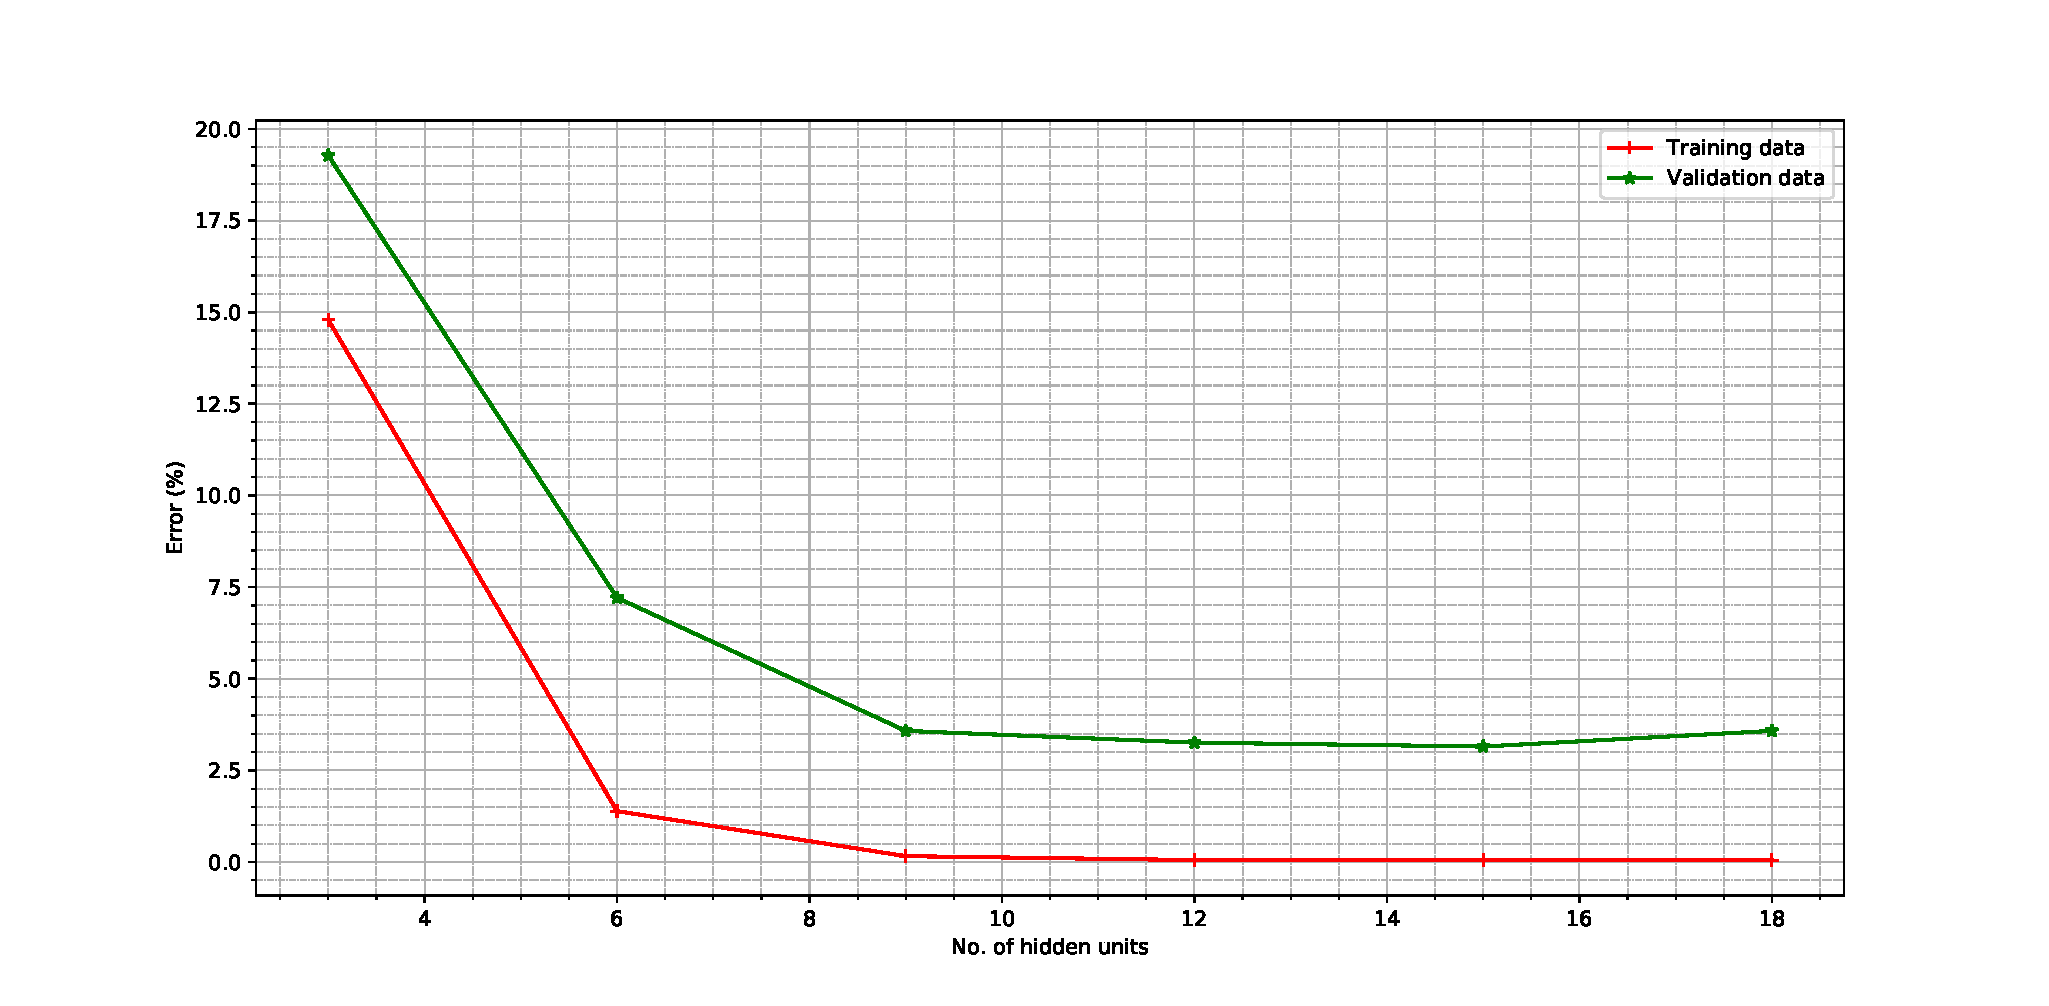
\includegraphics[scale=0.5]{2a_tv_error.pdf}
	\caption{Error Vs. hidden units plot for Optdigits training and validation data}
	\label{fig:tv_error_2a}
\end{figure}
\newline
As we can see from Fig.~\ref{fig:tv_error_2a}, both training and validation error decreases with increase in number of hidden units. But error on validation data with 18 hidden units gets slightly higher compared to 15 hidden units. This implies over-trained MLP. Therefore, for best results, we should choose 15 hidden units.

Error rate on test data with 15 hidden units is shown in the following table:
\begin{table}[h!]
	\begin{center}
		\begin{tabular}{||c | c ||} 
			\hline
			Hidden units & 15 \\ [0.5ex] 
			\hline\hline
			Test error(\%) & 4.1\\ [1ex]
			\hline
		\end{tabular}
	\end{center}
	\caption{Q2.a: Error-rate on test data}
\end{table}
%----------------------------------------------------------------------------------------
%	SOLUTION 2.b
%----------------------------------------------------------------------------------------
\subsection*{Solution 2.b}
Hidden units used = 15. Hidden representation with 2 principal components is shown in Fig.~\ref{fig:pca2_2b}, and with 3 principal components is shown in Fig.~\ref{fig:pca3_2b}.
\begin{figure}[h!]
	\centering
	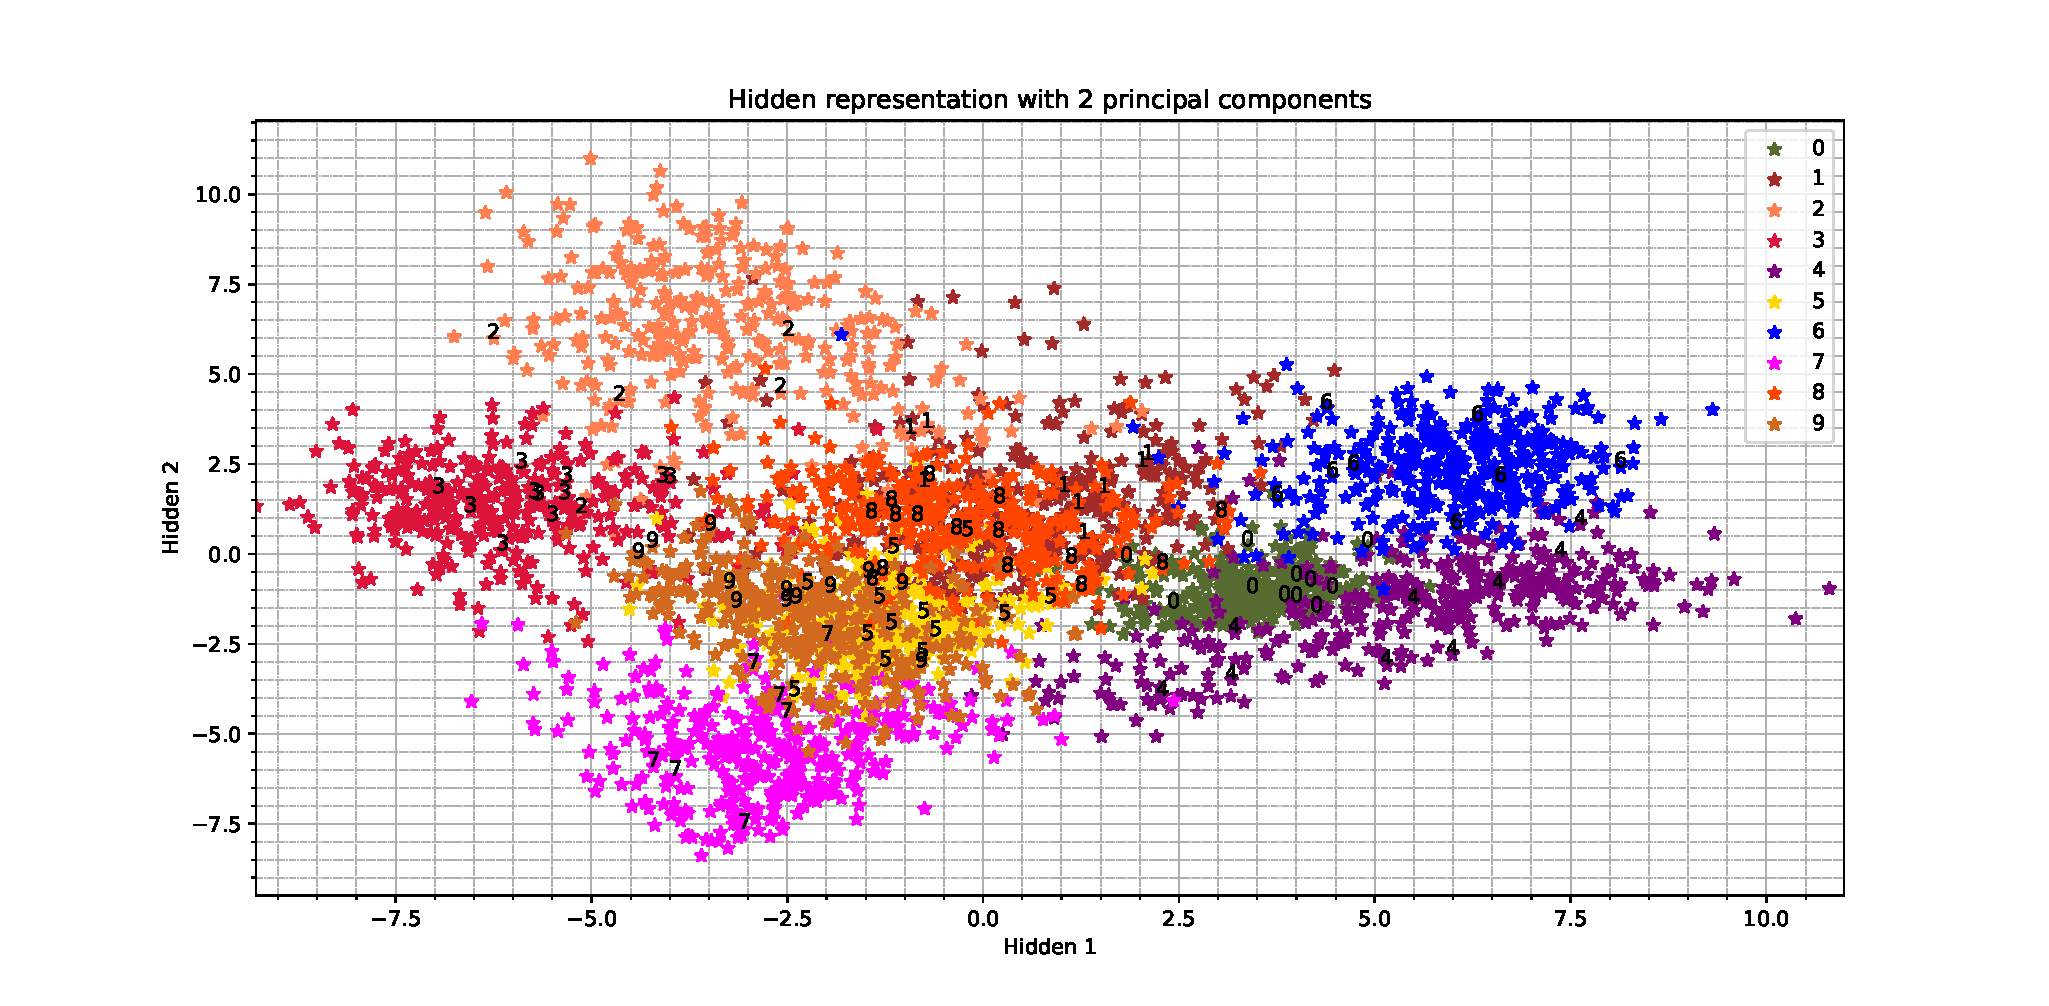
\includegraphics[scale=0.5]{2b_pca2.pdf}
	\caption{Hidden representation with 2 principal components on training and validation data}
	\label{fig:pca2_2b}
\end{figure}
\begin{figure}[h!]
	\centering
	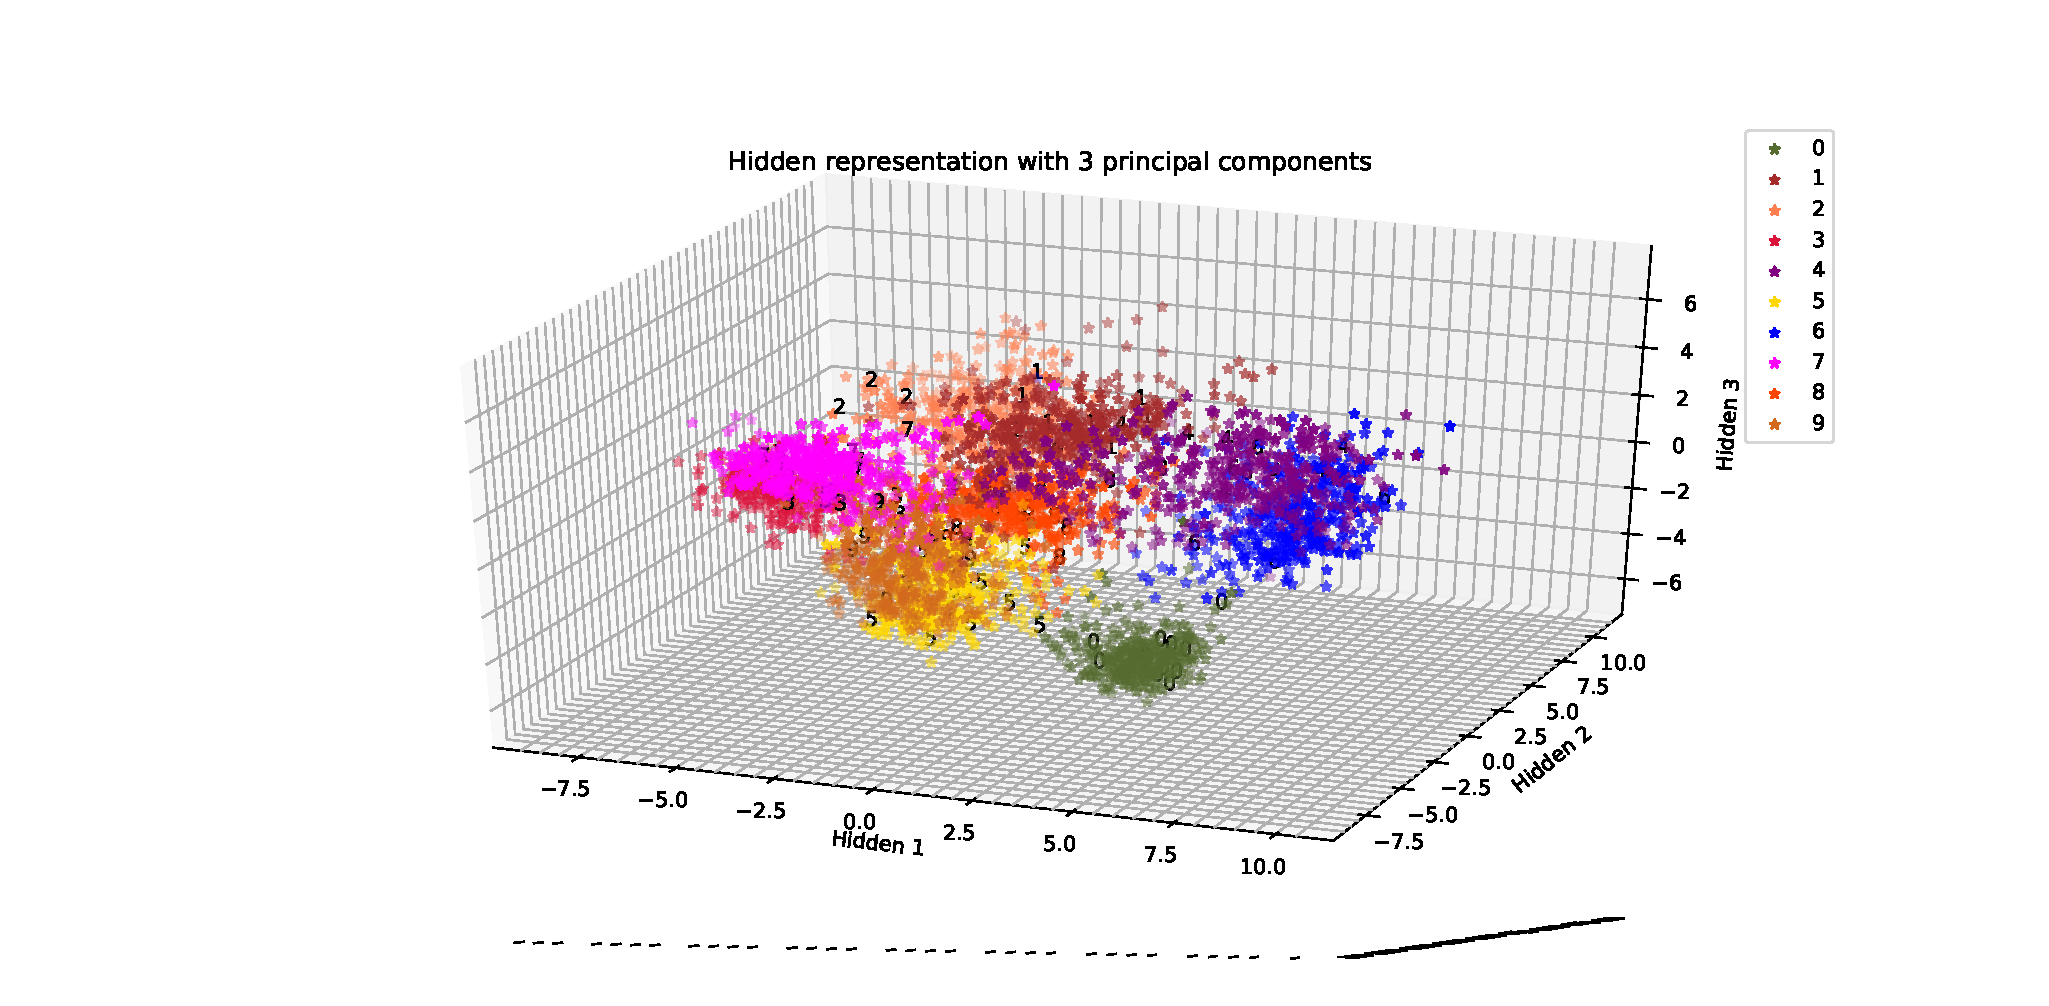
\includegraphics[scale=0.5]{2b_pca3.pdf}
	\caption{Hidden representation with 3 principal components on training and validation data}
	\label{fig:pca3_2b}
\end{figure}
Thus from Fig.~\ref{fig:pca2_2b} and Fig.~\ref{fig:pca3_2b}, we can see that PCA with 3 principal components provide better separation than with 2 principal components. This happens as number of PCA components behaves as a representation of number of units in the hidden layer.